% Source for paper_images/main_figure.pdf (Figure 1 of the CSUR manuscript).
% Three parallel signal columns feeding a single agentic system. Deliberately
% NO lifecycle-loop arrows and NO stage ordering: the three roles classify
% signals, not system stages (reviewer Q27s-3 / pqAY terminology point).
% Rebuild with: pdflatex main_figure_src.tex && mv main_figure_src.pdf main_figure.pdf
\documentclass[tikz,border=4pt]{standalone}
\usepackage{tikz}
\usetikzlibrary{positioning,arrows.meta}
\usepackage[T1]{fontenc}
\usepackage{helvet}
\renewcommand{\familydefault}{\sfdefault}

\definecolor{groundfill}{RGB}{218,232,252}
\definecolor{grounddraw}{RGB}{108,142,191}
\definecolor{delibfill}{RGB}{248,206,204}
\definecolor{delibdraw}{RGB}{184,84,80}
\definecolor{learnfill}{RGB}{255,242,204}
\definecolor{learndraw}{RGB}{214,182,86}
\definecolor{agentfill}{RGB}{245,245,245}
\definecolor{agentdraw}{RGB}{102,102,102}

\begin{document}
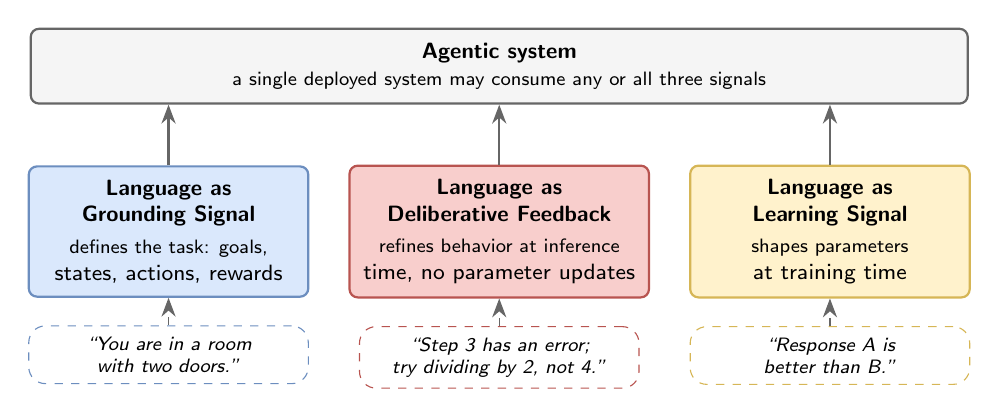
\begin{tikzpicture}[
  font=\footnotesize,
  pillar/.style={rounded corners=3pt, draw, thick, align=center,
                 minimum width=3.55cm, minimum height=1.55cm, inner sep=5pt},
  example/.style={rounded corners=6pt, draw, dashed, thin, align=center,
                  minimum width=3.55cm, inner sep=4pt, font=\scriptsize\itshape},
  sig/.style={-{Stealth[length=2.4mm]}, thick, draw=agentdraw}
]

% Top: the single system that consumes the signals
\node[pillar, fill=agentfill, draw=agentdraw, minimum width=11.9cm,
      minimum height=0.95cm] (agent) at (0,2.1)
  {\textbf{Agentic system}\\
   \scriptsize a single deployed system may consume any or all three signals};

% Three parallel signal columns (no ordering, no loop)
\node[pillar, fill=groundfill, draw=grounddraw] (ground) at (-4.2,0)
  {\textbf{Language as}\\ \textbf{Grounding Signal}\\[2pt]
   \scriptsize defines the task: goals,\\ states, actions, rewards};

\node[pillar, fill=delibfill, draw=delibdraw] (delib) at (0,0)
  {\textbf{Language as}\\ \textbf{Deliberative Feedback}\\[2pt]
   \scriptsize refines behavior at inference\\ time, no parameter updates};

\node[pillar, fill=learnfill, draw=learndraw] (learn) at (4.2,0)
  {\textbf{Language as}\\ \textbf{Learning Signal}\\[2pt]
   \scriptsize shapes parameters\\ at training time};

% Example utterances
\node[example, draw=grounddraw, below=0.35cm of ground] (gex)
  {``You are in a room\\ with two doors.''};
\node[example, draw=delibdraw, below=0.35cm of delib] (dex)
  {``Step 3 has an error;\\ try dividing by 2, not 4.''};
\node[example, draw=learndraw, below=0.35cm of learn] (lex)
  {``Response A is\\ better than B.''};

% Signals flow into the system; columns are not connected to each other
\draw[sig] (ground.north) -- (ground.north |- agent.south);
\draw[sig] (delib.north) -- (delib.north |- agent.south);
\draw[sig] (learn.north) -- (learn.north |- agent.south);
\draw[sig, dashed, thin] (gex.north) -- (ground.south);
\draw[sig, dashed, thin] (dex.north) -- (delib.south);
\draw[sig, dashed, thin] (lex.north) -- (learn.south);

\end{tikzpicture}
\end{document}
